\section{Experimental results}\label{sec:results}

To give comparative results on the quality of the initialisation processes
considered in this work, four well-known, categorical, labelled datasets ---
breast cancer, mushroom, nursery, and soybean (large) --- will be clustered by
the \(k\)-modes algorithm with each of the initialisation processes. These
datasets have been chosen to fall in line with the established literature, and
for their relative sizes and complexities. Each dataset is openly available
under the UCI Machine Learning Repository~\cite{Dua2019}, and their
characteristics are summarised in Table~\ref{tab:dataset_summary}. For the
purposes of this analysis, incomplete instances (i.e.\ where data is missing)
are excluded and the remaining dataset characteristics are reported as
`adjusted'.

\begin{table}[htbp]
    \resizebox{\textwidth}{!}{%
        \begin{tabular}{lrrrlrr}
\toprule
{} &  No. rows &  No. cols &  No. classes &  Missing values &  Adjusted no. rows &  Adjusted no. classes \\
\midrule
Breast cancer &       699 &        10 &            2 &            True &                683 &                     2 \\
Mushroom      &      8124 &        22 &            2 &            True &               5644 &                     2 \\
Soybean       &       307 &        35 &           19 &            True &                266 &                    15 \\
Nursery       &     12960 &         8 &            5 &           False &              12960 &                     5 \\
\bottomrule
\end{tabular}

    }\caption{A summary of the benchmark datasets.}\label{tab:dataset_summary}
\end{table}

Clustering algorithms are often evaluated based on their performance as a
classifier~\cite{%
    Arthur2007,Cao2009,Cao2012,Huang1998,%
    Ng2007,Olaode2014,Schaeffer2007,Sharma2015%
}. This is a fundamentally flawed approach --- especially given that
classification belongs to an entirely different branch of learning.  Moreover,
doing so requires a number of assumptions about the topology of the data within
the metric space that is being considered~\cite{Memoli2011}.  One such
assumption is that the classes recorded in the data are indeed separable objects
like clusters. The soybean dataset acts as an example where the labels attached
to the dataset may be too fine with respect to the space in which the data
exists. That is, in this case, only 8 clusters were identified from a possible
15 classes. This indicates that some of the classes are not easily distinguished
from one another. Likewise with the remaining datasets, an increase in the
number of clusters on the number of classes could suggest that the classes are
too vague or at the very least that more structure exists in the data than is
imposed. In any case, the choice of \(k\) when clustering is of great importance
and should strike a balance between explaining structure in the data and
interpretability of a model.

This analysis does not consider evaluative metrics related to classification
such as accuracy, recall or precision. Instead, only internal measures are
considered such as the cost function defined in~\eqref{eq:cost}. This metric is
label-invariant and its values are comparable across the different
initialisation methods. Furthermore, the effect of each initialisation method
on the initial and final clusterings can be captured with the cost function. An
additional, and often useful, metric is the silhouette coefficient. This
measures the ratio between the intra-cluster cohesion and inter-cluster
separation of a particular clustering. Therefore, it could be used in a similar
way to reveal the effect of each initialisation method at the beginning and end
of a run of \(k\)-modes. Unfortunately, this metric loses its intuition under
the distance measure employed here and is omitted. The remaining performance
measures used are the number of iterations for the \(k\)-modes algorithm to
terminate and the time taken to terminate in seconds.

The final piece of information required in this analysis is a choice for \(k\)
for each dataset. An immediate choice is the number of classes that are present
in a dataset but, as stated above, this is not necessarily a fair or wise choice
since the classes may not be representative of true clusters. A popular strategy
for choosing an optimal number of clusters is known as the `elbow' method. The
aim of this method is to identify a kink (elbow) in a plot of number of clusters
against cost for a dataset. Figure~\ref{fig:nursery_costs} is an example of such
a plot for the nursery dataset. This kink suggests that an increase in \(k\)
from there would not sufficiently improve the performance of the model. On its
own, this method is vague and somewhat unreliable which raises a number of
questions:
\begin{itemize}
    \item What constitutes a kink?
    \item How does one discern between multiple kinks?
    \item Is choosing a particular kink subjective to the observer?
\end{itemize}

\begin{figure}
    \centering
    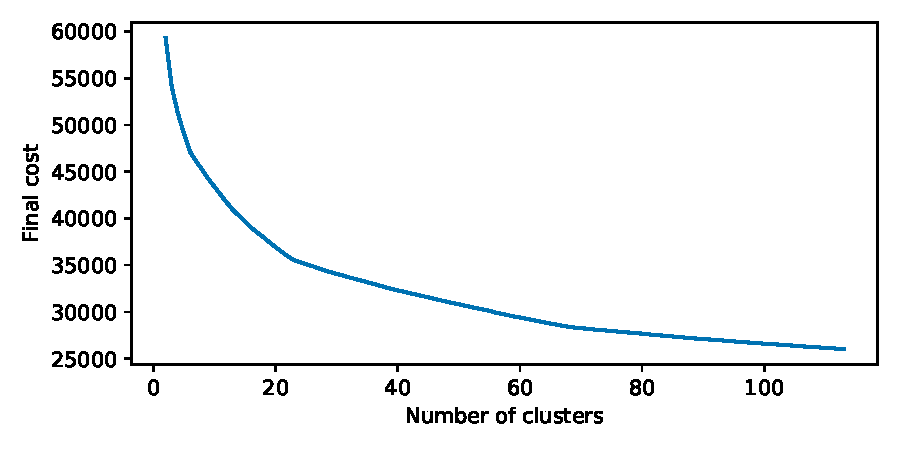
\includegraphics[width=.8\linewidth]{./img/elbow/nursery_costs.pdf}
    \caption{An elbow plot for the nursery dataset using Cao's initialisation
             method.}\label{fig:nursery_costs}
\end{figure}

An alternative `elbow' may be identified objectively by using the knee point
detection algorithm~\cite{Satopaa2011} where the maximal value of \(k\) is taken
to be \(\lfloor\sqrt{N}\rfloor\). This algorithm identifies the value of \(k\)
with the maximum curvature in the plot described above by computation rather
than inspection --- eliminating the concerns raised.

\subsection{Elbow method}\label{subsec:elbow}
\graphicspath{{./img/elbow/}}

Tables~\ref{tab:breast_cancer_elbow}---\ref{tab:soybean_elbow}
summarise the results of each initialisation method on the benchmark datasets
where the number of clusters has been determined by the knee point detection
algorithm. Each column shows the mean value of each metric and its standard
deviation in parentheses over 250
independent
repetitions of the \(k\)-modes algorithm.

\begin{table}[htbp]
    \centering
    \resizebox{\tablewidth}{!}{%
        \begin{tabular}{lllll}
\toprule
{} &      Initial cost &        Final cost & No. iterations &          Time \\
\midrule
Cao      &   2178.00 (0.000) &   1955.00 (0.000) &   4.00 (0.000) &  0.37 (0.025) \\
Huang    &  2123.12 (92.805) &  2023.80 (49.390) &   2.58 (0.810) &  0.25 (0.054) \\
Matching &  2110.68 (87.670) &  2015.42 (40.354) &   2.72 (0.834) &  0.21 (0.034) \\
\bottomrule
\end{tabular}

    }
    \captionof{table}{Summative metric results for the breast cancer dataset
    with \(k=8\).}\label{tab:breast_cancer_elbow}\vspace{20pt}

    \resizebox{\tablewidth}{!}{%
        \begin{tabular}{lllll}
\toprule
{} &         Initial cost &           Final cost & No. iterations &          Time \\
\midrule
Cao      &     29922.00 (0.000) &     29621.00 (0.000) &   2.00 (0.000) &  1.78 (0.066) \\
Huang    &  35112.67 (3286.612) &  31312.27 (1387.005) &   2.98 (1.012) &  2.74 (0.758) \\
Matching &  35237.67 (3201.877) &  31183.28 (1143.908) &   2.99 (0.924) &  1.79 (0.421) \\
\bottomrule
\end{tabular}

    }
    \captionof{table}{Summative metric results for the mushroom dataset with
    \(k=17\).}\label{tab:mushroom_elbow}\vspace{20pt}

    \resizebox{\tablewidth}{!}{%
        \begin{tabular}{lllll}
\toprule
{} &        Initial cost &          Final cost & No. iterations &          Time \\
\midrule
Cao      &    35544.00 (0.000) &    35544.00 (0.000) &   1.00 (0.000) &  4.98 (0.152) \\
Huang    &  37535.06 (372.596) &  37535.06 (372.596) &   1.00 (0.000) &  3.58 (0.121) \\
Matching &  37484.29 (327.467) &  37484.29 (327.467) &   1.00 (0.000) &  3.14 (0.141) \\
\bottomrule
\end{tabular}

    }
    \captionof{table}{Summative metric results for the nursery dataset with
    \(k=23\).}\label{tab:nursery_elbow}\vspace{20pt}

    \resizebox{\tablewidth}{!}{%
        \begin{tabular}{lllll}
\toprule
{} &       Initial cost &        Final cost & No. iterations &          Time \\
\midrule
Cao      &    1822.00 (0.000) &   1700.00 (0.000) &   4.00 (0.000) &  0.24 (0.009) \\
Huang    &  1964.56 (107.504) &  1832.92 (61.820) &   3.36 (0.875) &  0.23 (0.043) \\
Matching &   1929.50 (85.928) &  1829.54 (68.632) &   3.44 (1.110) &  0.15 (0.027) \\
\bottomrule
\end{tabular}

    }
    \captionof{table}{Summative metric results for the soybean dataset with
    \(k=8\).}\label{tab:soybean_elbow}
\end{table}

By examining these tables it would seem that the proposed method and Huang's
method are comparable across the board --- although the proposed method is
faster despite taking more iterations in general. More importantly though, it
appears that Cao's method performs the best out of the three initialisation
methods: in terms of initial and final costs Cao's method improves, on average,
by roughly 10 percent against the next best method for the three datasets that
it succeeds with; the number of iterations is comparable; and the computation
time is substantially less than the other two considering it is a deterministic
method and need only be run once to achieve this performance.

However, in the \(k\)-means paradigm, a particular clustering is selected based
on it having the minimum final cost over a number of runs of the algorithm ---
not the mean --- and while Cao's method is very reliable, in that there is no
variation at all, it does not always produce the best clustering possible. There
is a trade-off to be made between computational time and performance here. In
order to gain more insight into the performance of each method, less granular
analysis is required.
Figures~\ref{fig:breast_cancer_elbow}---\ref{fig:soybean_elbow} display the
cost function results for each dataset in the form of a scatter plot and two
empirical cumulative density function (CDF) plots, highlighting the breadth and
depth of the behaviours exhibited by each initialisation method.

Looking at Figure~\ref{fig:breast_cancer_elbow} it is clear that in terms of
final cost Cao's method is middling when compared to the other methods. This
was apparent from Table~\ref{tab:breast_cancer_elbow} and, indeed, Huang's and
the proposed method are both very comparable when looking at the main body of
the results. However, since the criterion for the best clustering (in practical
terms) is having the minimum final cost, it is evident that the proposed method
is superior; that the method produces clusterings with a larger cost
range (indicated by the trailing right-hand side of each CDF plot) is irrelevant
for the same reason.

This pattern of largely similar behaviour between Huang's and the proposed
method is apparent in each of the figures here, and in each case the proposed
method outperforms Huang's. In fact, in all cases except for the nursery
dataset, the proposed method achieves the lowest final cost of all the methods
and, as such, performs the best in practical terms on these particular datasets.

In the case of the nursery dataset, Cao's method is unquestionably the best
performing initialisation method. It should be noted that none of the
methods were able to find an initial clustering that could be improved on, and
that this dataset exactly describes the entire attribute space in which it
exists. This property could be why the other methods fall behind Cao's so
decisively in that Cao's method is able to definitively choose the \(k\) most
dense-whilst-separated points from the attribute space as the initial cluster
centres whereas the other two methods are in essence randomly sampling from this
space. That each initial solution in these repetitions is locally optimal
remains a mystery.

\begin{figure}
    \begin{subfigure}{.5\textwidth}
        \includegraphics[width=\linewidth]%
            {breast_cancer_cost_scatterplot.pdf}
        \caption{Scatter plot of initial and final costs.}
    \end{subfigure}
    \hfill%
    \begin{subfigure}{.5\textwidth}
        \includegraphics[width=\linewidth]%
            {breast_cancer_initial_cost_cdfplot.pdf}

            \includegraphics[width=\linewidth]%
            {breast_cancer_final_cost_cdfplot.pdf}
        \caption{Empirical CDF plots for initial (top) and final (bottom)
                 costs.}
    \end{subfigure}
    \caption{Summative plots for the breast cancer dataset with \(k=8\).}%
    \label{fig:breast_cancer_elbow}
\end{figure}

\begin{figure}
    \begin{subfigure}{.5\textwidth}
        \includegraphics[width=\linewidth]%
            {mushroom_cost_scatterplot.pdf}
        \caption{Scatter plot of initial and final costs.}
    \end{subfigure}
    \hfill%
    \begin{subfigure}{.5\textwidth}
        \includegraphics[width=\linewidth]%
            {mushroom_initial_cost_cdfplot.pdf}
        
        \includegraphics[width=\linewidth]%
            {mushroom_final_cost_cdfplot.pdf}
        \caption{Empirical CDF plots for initial (top) and final (bottom)
                 costs.}
    \end{subfigure}
    \caption{Summative plots for the mushroom dataset with \(k=17\).}%
    \label{fig:mushroom_elbow}
\end{figure}

\begin{figure}
    \begin{subfigure}{.5\textwidth}
        \includegraphics[width=\linewidth]%
            {nursery_cost_scatterplot.pdf}
        \caption{Scatter plot of initial and final costs.}
    \end{subfigure}
    \hfill%
    \begin{subfigure}{.5\textwidth}
        \includegraphics[width=\linewidth]%
            {nursery_initial_cost_cdfplot.pdf}

        \includegraphics[width=\linewidth]%
            {nursery_final_cost_cdfplot.pdf}
        \caption{Empirical CDF plots for initial (top) and final (bottom)
                 costs.}
    \end{subfigure}
    \caption{Summative plots for the nursery dataset with \(k=23\).}%
    \label{fig:nursery_elbow}
\end{figure}

\begin{figure}
    \begin{subfigure}{.5\textwidth}
        \includegraphics[width=\linewidth]%
            {soybean_cost_scatterplot.pdf}
        \caption{Scatter plot of initial and final costs.}
    \end{subfigure}
    \hfill%
    \begin{subfigure}{.5\textwidth}
        \includegraphics[width=\linewidth]%
            {soybean_initial_cost_cdfplot.pdf}

        \includegraphics[width=\linewidth]%
            {soybean_final_cost_cdfplot.pdf}
        \caption{Empirical CDF plots for initial (top) and final (bottom)
                 costs.}
    \end{subfigure}
    \caption{Summative plots for the soybean dataset with \(k=8\).}%
    \label{fig:soybean_elbow}
\end{figure}


\subsection{Number of classes}
\graphicspath{{./img/nclasses/}}

As is discussed above, the often automatic choice for \(k\) is the number of
classes present in the data; this subsection repeats the analysis as with the
elbow method but with this traditional choice for \(k\).
Tables~\ref{tab:breast_cancer_nclasses}---\ref{tab:soybean_nclasses}
contain the analogous summaries of each initialisation method's performance on
the benchmark datasets over the same number of repetitions.

\begin{table}[htbp]
    \centering
    \resizebox{\tablewidth}{!}{%
        \begin{tabular}{lllll}
\toprule
{} &       Initial cost &         Final cost & No. iterations &          Time \\
\midrule
Cao      &    3315.00 (0.000) &    3172.00 (0.000) &   2.00 (0.000) &  0.13 (0.005) \\
Huang    &  3393.80 (120.772) &  3348.51 (144.849) &   1.54 (0.653) &  0.10 (0.024) \\
Matching &  3406.73 (111.686) &  3355.56 (144.621) &   1.61 (0.638) &  0.09 (0.018) \\
\bottomrule
\end{tabular}

    }
    \captionof{table}{Summative metric results for the breast cancer dataset
    with \(k=2\).}\label{tab:breast_cancer_nclasses}\vspace{20pt}

    \resizebox{\tablewidth}{!}{%
        \begin{tabular}{lllll}
\toprule
{} &         Initial cost &           Final cost & No. iterations &          Time \\
\midrule
Cao      &     37662.00 (0.000) &     37662.00 (0.000) &   1.00 (0.000) &  1.10 (0.142) \\
Huang    &  41720.20 (2519.647) &  38612.64 (2086.246) &   3.14 (1.471) &  2.04 (0.759) \\
Matching &  42297.98 (2265.532) &  39496.56 (2681.581) &   3.36 (1.439) &  1.62 (0.567) \\
\bottomrule
\end{tabular}

    }
    \captionof{table}{Summative metric results for the mushroom dataset with
    \(k=2\).}\label{tab:mushroom_nclasses}\vspace{20pt}

    \resizebox{\tablewidth}{!}{%
        \begin{tabular}{lllll}
\toprule
{} &        Initial cost &          Final cost & No. iterations &          Time \\
\midrule
Cao      &    49060.00 (0.000) &    49060.00 (0.000) &   1.00 (0.000) &  1.80 (0.090) \\
Huang    &  51229.45 (902.503) &  51229.45 (902.503) &   1.00 (0.000) &  1.72 (0.116) \\
Matching &  51107.52 (910.258) &  51101.95 (903.525) &   1.00 (0.063) &  1.37 (0.128) \\
\bottomrule
\end{tabular}

    }
    \captionof{table}{Summative metric results for the nursery dataset with
    \(k=5\).}\label{tab:nursery_nclasses}\vspace{20pt}

    \resizebox{\tablewidth}{!}{%
        \begin{tabular}{lllll}
\toprule
{} &      Initial cost &        Final cost & No. iterations &          Time \\
\midrule
Cao      &   1364.00 (0.000) &   1314.00 (0.000) &   2.00 (0.000) &  0.35 (0.043) \\
Huang    &  1586.90 (83.851) &  1444.56 (58.788) &   4.03 (1.114) &  0.46 (0.085) \\
Matching &  1585.66 (88.345) &  1447.63 (59.620) &   4.04 (1.123) &  0.24 (0.022) \\
\bottomrule
\end{tabular}

    }
    \captionof{table}{Summative metric results for the soybean dataset with
    \(k=15\).}\label{tab:soybean_nclasses}
\end{table}

An immediate comparison to the previous tables is that for all datasets bar the
soybean dataset, the mean costs are significantly higher and the computation
times are lower. These effects come directly from the choice of \(k\) in that
higher values of \(k\) will require more checks (and thus computational time)
but will typically lead to more homogeneous clusters, reducing their
within-cluster dissimilarity and therefore cost.

Looking at these tables on their own, Cao's method is the superior
initialisation method on average: the means are substantially lower in terms of
initial and final cost; there is no deviation in these results; again, the total
computational time is a fraction of the other two methods. It is also apparent
that Huang's method and the proposed extension are very comparable on average.
As before, finer investigation will require finer visualisations.
Figures~\ref{fig:breast_cancer_nclasses}---\ref{fig:soybean_nclasses} show the
same plots as in the previous subsection except the number of clusters has been
taken to be the number of classes present in each dataset.

Figures~\ref{fig:breast_cancer_nclasses}~\&~\ref{fig:mushroom_nclasses} indicate
that a particular behaviour emerged during the runs of the \(k\)-modes
algorithm. Specifically, each solution falls into one of (predominantly) two
types: effectively no improvement on the initial clustering, or terminating at
some clustering with a cost that is bounded below across all such solutions.
Invariably, Cao's method achieves this lower bound and unless Cao's method is
used, these particular choices for \(k\) mean that the performance of the
\(k\)-modes algorithm is exceptionally sensitive to its initial clustering.
Moreover, the other two methods are effectively indistinguishable in these
cases and so if a robust solution is required, Cao's method is the only viable
option.

Another point to be raised from these two figures is that the \(k\)-modes
algorithm is susceptible to a worsening move between iterations. This may seem
counter-intuitive but is possible since the cluster centres are updated after
every point is moved rather than at the end of the iteration. That is, a move
that may be beneficial when moving a point between clusters may not be
beneficial to the cluster overall in terms of within-cluster dissimilarity by
the end of an iteration.

Figure~\ref{fig:nursery_nclasses} corresponds to the nursery dataset with
\(k~=~5\). In this set of runs, the same pattern emerges where sampling the
initial centres from amongst the most dense points (via Huang's method and the
proposed) is an inferior strategy to one considering the entire attribute space
such as with Cao's method. Again, no method is able to improve on the initial
solution except for one repetition with the matching initialisation method.

\begin{figure}
    \begin{subfigure}{.5\textwidth}
        \includegraphics[width=\linewidth]%
            {breast_cancer_cost_scatterplot.pdf}
        \caption{Scatter plot of initial and final costs.}
    \end{subfigure}
    \hfill%
    \begin{subfigure}{.5\textwidth}
        \includegraphics[width=\linewidth]%
            {breast_cancer_initial_cost_cdfplot.pdf}

        \includegraphics[width=\linewidth]%
            {breast_cancer_final_cost_cdfplot.pdf}
        \caption{Empirical CDF plots for initial (top) and final (bottom)
                 costs.}
    \end{subfigure}
    \caption{Summative plots for the breast cancer dataset with \(k=2\).}%
    \label{fig:breast_cancer_nclasses}
\end{figure}

\begin{figure}
    \begin{subfigure}{.5\textwidth}
        \includegraphics[width=\linewidth]%
            {mushroom_cost_scatterplot.pdf}
        \caption{Scatter plot of initial and final costs.}
    \end{subfigure}
    \hfill%
    \begin{subfigure}{.5\textwidth}
        \includegraphics[width=\linewidth]%
            {mushroom_initial_cost_cdfplot.pdf}

        \includegraphics[width=\linewidth]%
            {mushroom_final_cost_cdfplot.pdf}
        \caption{Empirical CDF plots for initial (top) and final (bottom)
                 costs.}
    \end{subfigure}
    \caption{Summative plots for the mushroom dataset with \(k=2\).}%
    \label{fig:mushroom_nclasses}
\end{figure}

\begin{figure}
    \begin{subfigure}{.5\textwidth}
        \includegraphics[width=\linewidth]%
            {nursery_cost_scatterplot.pdf}
        \caption{Scatter plot of initial and final costs.}
    \end{subfigure}
    \hfill%
    \begin{subfigure}{.5\textwidth}
        \includegraphics[width=\linewidth]%
            {nursery_initial_cost_cdfplot.pdf}

        \includegraphics[width=\linewidth]%
            {nursery_final_cost_cdfplot.pdf}
        \caption{Empirical CDF plots for initial (top) and final (bottom)
                 costs.}
    \end{subfigure}
    \caption{Summative plots for the nursery dataset with \(k=5\).}%
    \label{fig:nursery_nclasses}
\end{figure}

\begin{figure}
    \begin{subfigure}{.5\textwidth}
        \includegraphics[width=\linewidth]%
            {soybean_cost_scatterplot.pdf}
        \caption{Scatter plot of initial and final costs.}
    \end{subfigure}
    \hfill%
    \begin{subfigure}{.5\textwidth}
        \includegraphics[width=\linewidth]%
            {soybean_initial_cost_cdfplot.pdf}

        \includegraphics[width=\linewidth]%
            {soybean_final_cost_cdfplot.pdf}
        \caption{Empirical CDF plots for initial (top) and final (bottom)
                 costs.}
    \end{subfigure}
    \caption{Summative plots for the soybean dataset with \(k=15\).}%
    \label{fig:soybean_nclasses}
\end{figure}

The primary conclusion from this analysis is that while Huang's method is
largely comparable to the proposed extension, there is no substantial evidence
from these use cases to use Huang's method over the one proposed in this work.
This is due to the proposed method performing better (or as well as) Huang's
in terms of minimal final costs and computational time over a number of runs in
both the cases where an external framework is imposed on the data (by choosing
\(k\) to be the number of classes) and not. Furthermore, though not discussed in
this work, the matching initialisation method has the scope to allow for expert
or prior knowledge to be included in an initial clustering by using a particular
preference list mechanism.
